\documentclass[11pt]{article}
\usepackage[a4paper,margin=2cm]{geometry}
\usepackage[brazilian]{babel}
\usepackage[utf8]{inputenc}
\usepackage[T1]{fontenc}
\linespread{1.3}
\parskip=12pt
\parindent=0pt
\usepackage{enumitem}
\usepackage{amsmath}
\usepackage{amsfonts}
\usepackage{graphicx}
\usepackage{amssymb}
\usepackage{hyperref}
\usepackage{amsthm}
\usepackage{color}


% Defining the question styles
\theoremstyle{definition}
\newtheorem{prob}{Problem}

\theoremstyle{definition}
\newtheorem{problema}{Problema}

% Custom commands
\newcommand{\E}{\mathbb{E}}
\newcommand{\Var}{\mathrm{Var}}
\newcommand{\Prob}{\mathbb{P}}

% declare a new theorem style
\newtheoremstyle{solution}%
{1pt}% Space above
{1pt}% Space below 
{\itshape\color{red}}% Body font
{}% Indent amount
{\bfseries\color{red}}% Theorem head font
{.}% Punctuation after theorem head
{.5em}% Space after theorem head
{}% Theorem head spec (can be left empty, meaning ‘normal’)

\theoremstyle{solution}
\newtheorem*{solution}{Solution}

% --- Code starts here ---
\begin{document}
	\begin{center}
		{\Large{\textbf{Lista II - Métodos Numéricos}}}\\
		\vspace{0.2cm}
		EPGE - 2018\\
		Professor: Cézar Santos\\
		Aluno: Raul Guarini Riva
	\end{center}

\begin{problema}
	O problema no planejador consiste em escolher recursivamente quanto consumir no presente e quanto poupar na forma de capital para o próximo período, tendo por base o estado da economia formado pelo estoque de capital atual e a produtividade atual. 
	
	A função utilidade das famílias não leva em consideração o lazer. Desta forma, ofertarão trabalho inelasticamente. Normalizando a dotação de trabalho para uma unidade, a equação funcional com a qual o planejador se defronta é a seguinte:
	\begin{gather*}
		V(K, z) = \max\limits_{c, K'} \{u(c) + \beta\E[V(K', z')|z] \} \\
		\text{s.t.} \quad c + K' \leq zK^{\alpha} + (1-\delta)K
	\end{gather*}
	
	A hipótese de $u$ estritamente crescente implica que a restrição de recursos será satisfeita com igualdade em todo instante do tempo. Daí, reescreve-se:
	\begin{gather*}
		V(K,z) = \max\limits_{K'}\{u(zK^{\alpha} + (1-\delta)K - K') + \beta\E[V(K', z')|z]\}
	\end{gather*}
\end{problema}

\begin{problema}
	Supondo não haver incerteza, normaliza-se o valor da produtividade para a média incondicional do processo:
	\begin{equation*}
		\log(z) = 0 \implies z = 1
	\end{equation*}
	
	A equação de Euler é dada por
	\begin{gather*}
		\beta\E\bigg[\left(\frac{c'}{c}\right)^{-\mu}(z'\alpha K'^{\alpha - 1} + 1 - \delta)\big|z\bigg] = 1
	\end{gather*}
	Sem incerteza e já resolvendo para o estado estacionário:
	\begin{gather*}
		\beta\alpha K^{\alpha -1}_{ss} = 1 - \beta(1-\delta)\\
		\boxed{K_{ss} = \left(\frac{\alpha\beta}{1 - \beta(1-\delta)} \right)^{\frac{1}{1-\alpha}}}
	\end{gather*}
	
	Com a calibração sugerida na lista, temos $K_{ss} = 48.1905$.
\end{problema}

\begin{problema}
	Para esta primeira implementação, explorei a monotonicidade da função política e a concavidade do funcional sendo otimizado. O código está no formato de uma função chamada \texttt{VFinder\_Iterated.m}, devidamente documentada através do próprio \texttt{help} do MATLAB.
	
	A primeira iteração foi feita através de força bruta e as próximas seguiram explorando os aspectos teóricos do problema. Abaixo, a função valor e a função política (como esperado, crescente!!!):
	\begin{figure}[htb!]
		\centering
		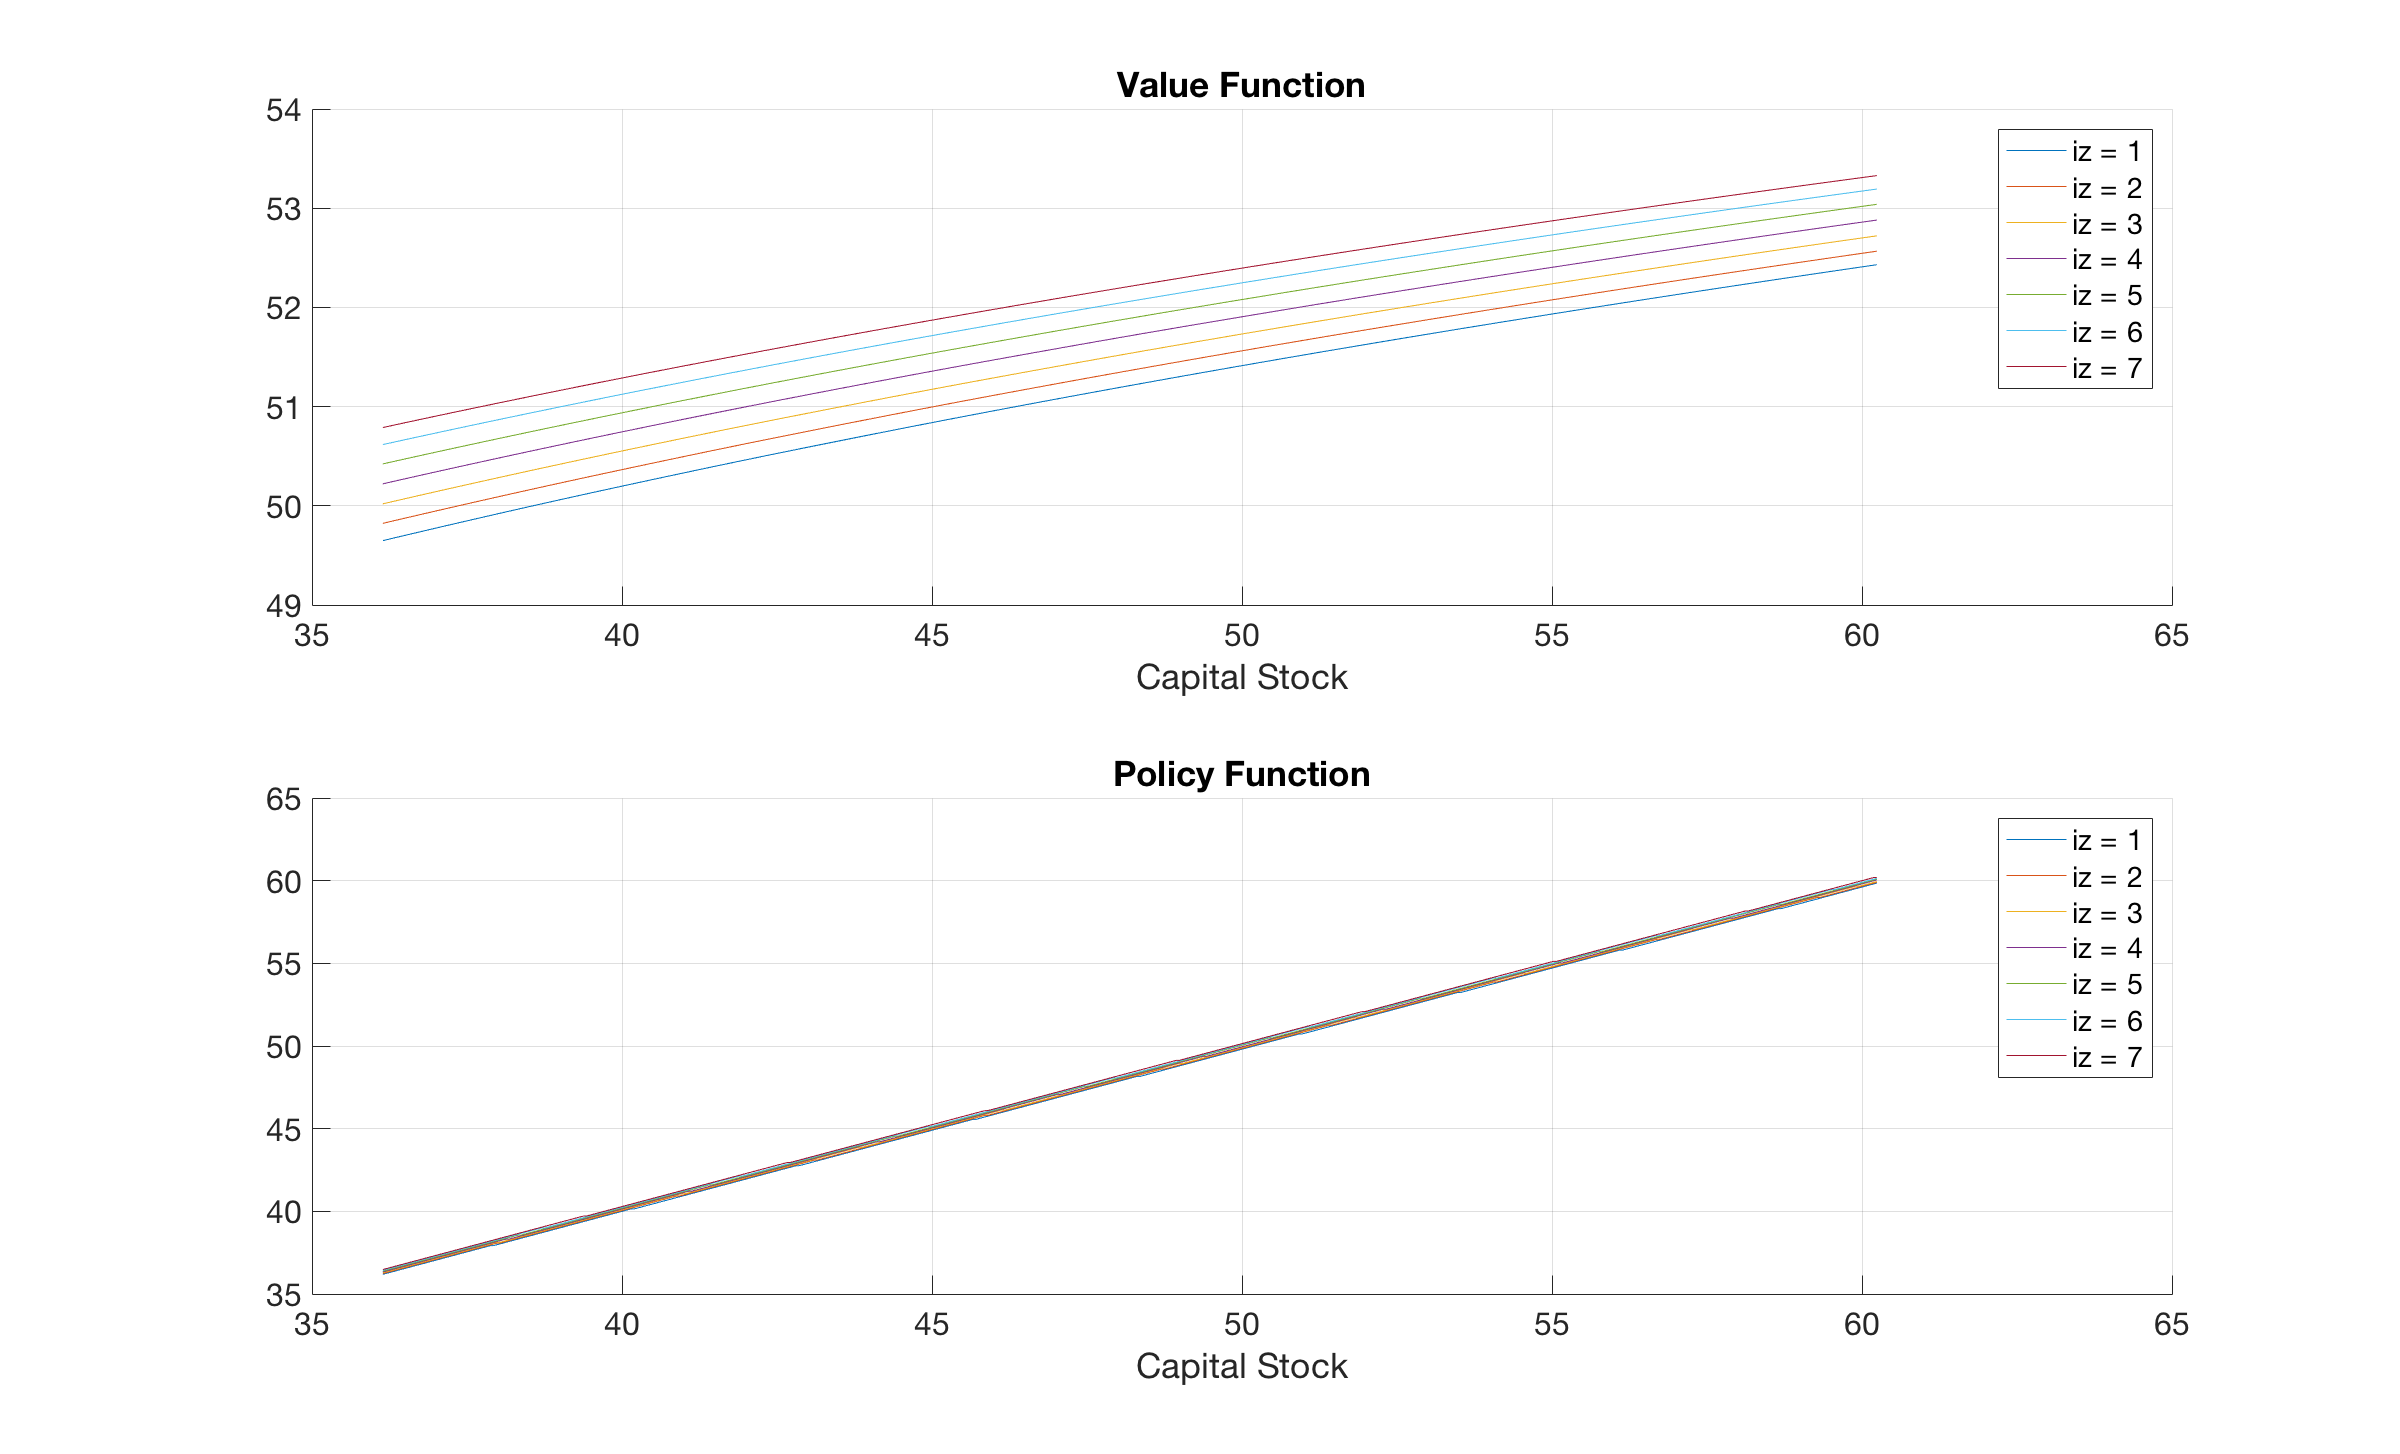
\includegraphics[scale = 0.22]{problem3_V_vs_G}
	\end{figure}
	
	Obtive o resultado, também esperado, de que a função valor, para um valor de $k$ fixo, é crescente na TFP. A legenda iz $= 4$, por exemplo, indica que determinada curva foi computada com o valor da TFP correspondente ao quarto ponto do grid do choque $\log (z)$.
	
	Para comparar o desempenho desta abordagem (que não utiliza nenhum tipo de vetorização), implementei o método de ``força bruta vetorizada''. Isto é, operar maximizações ao longo das dimensões de arrays do MATLAB evitando criar ``for loops''. Esta abordagem está no script \texttt{brute\_force.m}.
	
	Houve um ganho de desempenho considerável. O método de força bruta vetorizada computou a função valor e a função política em 9.96 segundos. O método que utiliza a função \texttt{VFinder\_Iterated.m} resolveu o mesmo problema em 7.84 segundos. Isto representa um ganho de quase 22\%, o que considero expressivo. 
	
	Nota-se, entretanto, que o método de força bruta é mais geral que seu concorrente, em vista do fato que funcionaria igualmente bem para um problema em que não tivéssemos um resultado teórico garantindo a monotonicidade da função política ou a concavidade do funcional em questão. Uma performance pior é o preço a ser pago pela maior versatilidade.
	\end{problema}
	
	\begin{problema}
		A função \texttt{VFinder\_Accelerated} implementa o mesmo algoritmo do problem anterior, se valendo da técnica do acelerador, contudo. Seu último argumento, \texttt{pct}, informa à função qual a frequência em que deve ser utilizada uma otimização completa: atualização da função política e da função valor. Por exemplo, \texttt{pct = 0.1} faz com que em 10\% das iterações só façamos a atualização da função valor, utilizando a função política de anterior. 
		
		Nas 50 primeiras iterações do algoritmo, otimizações completas são feitas, com o objetivo de colocar o processo ``na rota de convergência'' (isto é controlado através do parâmetro \texttt{safety\_net} no escopo da função).
		
		Abaixo, uma comparação das funções valor encontradas. Como esperado, temos a mesma solução (a menos de erros de aritmética de ponto flutuante):
		\begin{figure}[h!]
			\centering
			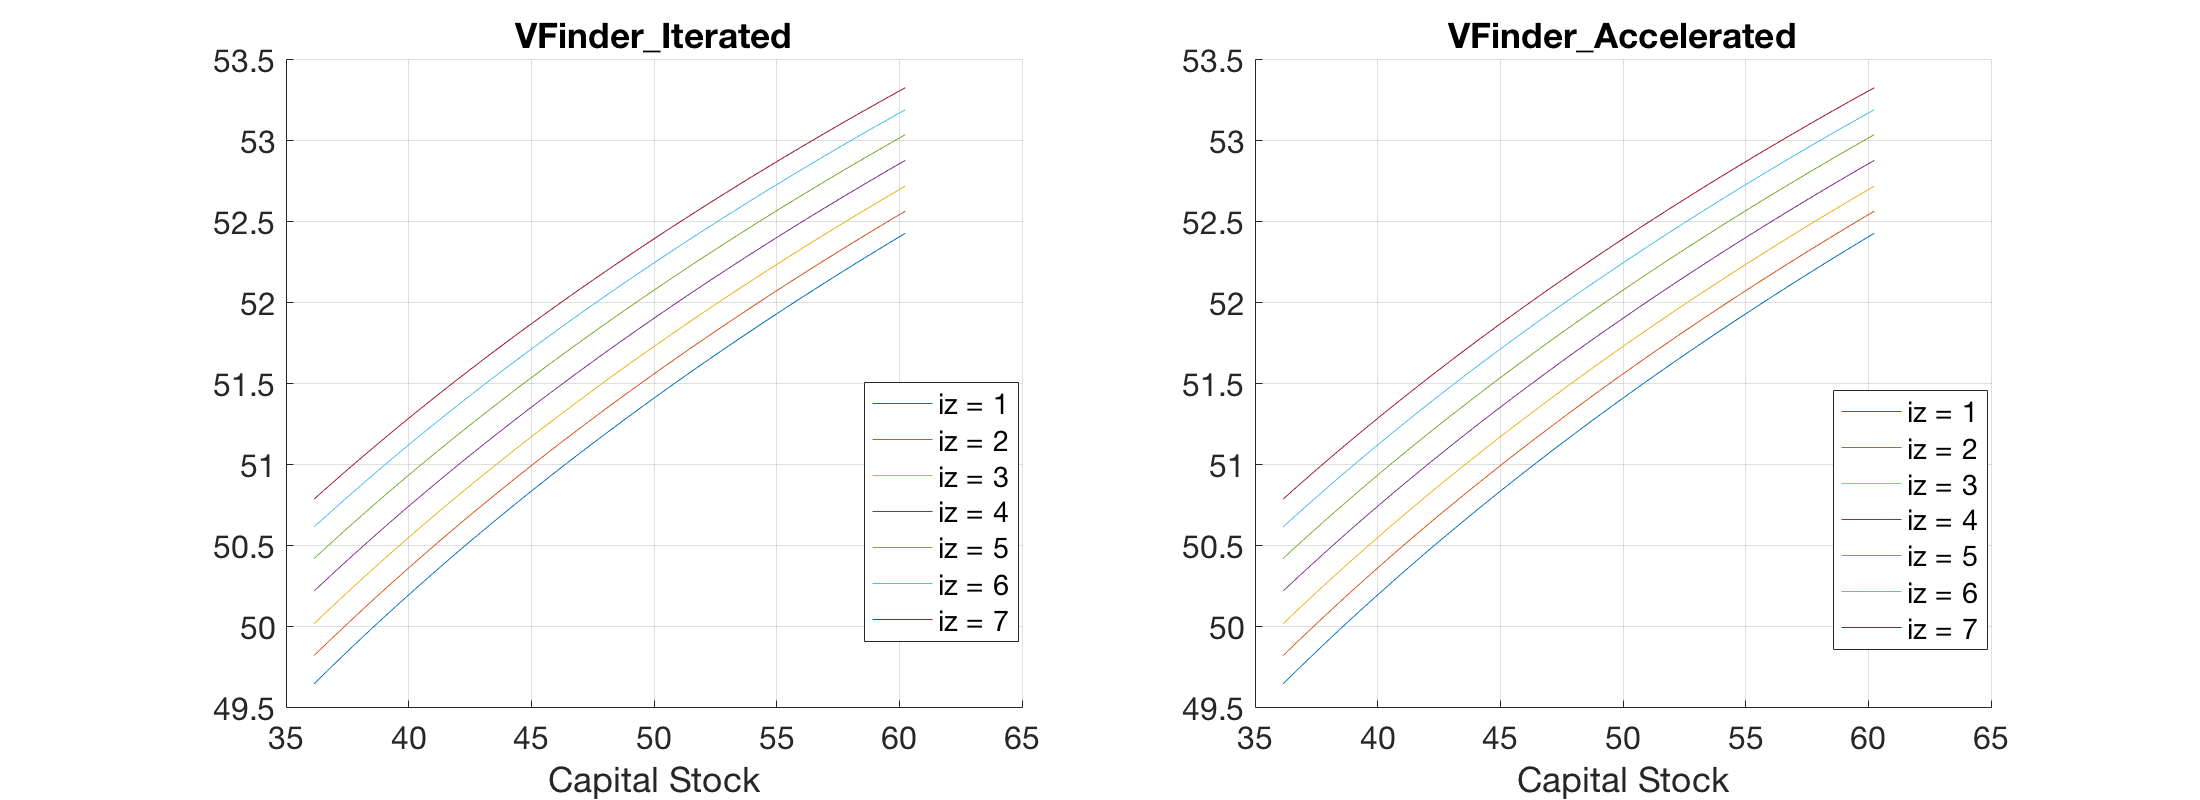
\includegraphics[scale = 0.2]{iterated_vs_accelerated}
		\end{figure}
		
		A função \texttt{VFinder\_Accelerated} resolveu o modelo em 7.66 segundos, cerca de 3\% mais rápido do que \texttt{VFinder\_Iterated}. O ganho de velocidade não foi expressivo, em minha visão, porque o algoritmo rival já não usa, a não ser na primeira iteração, o operador $\max()$, em vista da maneira como a concavidade do funcional foi explorada. Isto reduz o ganho de performance potencial do acelerador. Quando comparamos esta solução com a implementação de força bruta, entretanto, notamos um ganho de performance de mais de 3 segundos, mais de 30\%!\footnote{Estes resultados foram computados com base na sugestão da lista de usar $\texttt{pct}= 0.1$.}
		
		
	\end{problema}
	
	
\begin{problema}
	O método do multigrid mostrou-se poderoso. Analisando o formato da função valor encontrada através dos outros dois métodos e em vista da facilidade/rapidez de sua implementação, optei pelo uso da interpolação linear. A curvatura de $V$ ao redor do estado estacionário não parece tão grande.
	
	Dado um chute inicial para a função valor, resolvi o problema funcional num grid inicial com 100 pontos, interpolei os valores encontrados num grid mais fino de 500 pontos e utilizei o interpolante como um novo chute inicial para resolver o problema no grid mais fino. Esta interpolação ocorreu linearmente para cada valor de $z$ fixo. Resolvido o problema no grid de 500 pontos, repeti o processo visando resolver a equação funcional num grid de 5000 pontos para $k$. O algoritmo levou ao redor de 73 segundos para convergir.
		
	Claro, este problema é mais complicado do que o problema anterior uma vez que multiplicamos por 10 o número de pontos no grid de $k$. Como discretizamos também a variável de controle, aumentamos em 100 vezes o número de pontos considerados. 
	
	Para comparar o desempenho do multigrid com os dois outros métodos implementados acima, através de \texttt{VFinder\_Iterated} e \texttt{VFinder\_Accelerated}, resolvi o problema com uma sequência de grids de 100, 250 e, finalmente, 500 pontos. O tempo de execução foi de 0.58 segundos, isto é, mais de 10x mais rápido do que os outros dois métodos!
	\begin{figure}[h!]
		\centering
		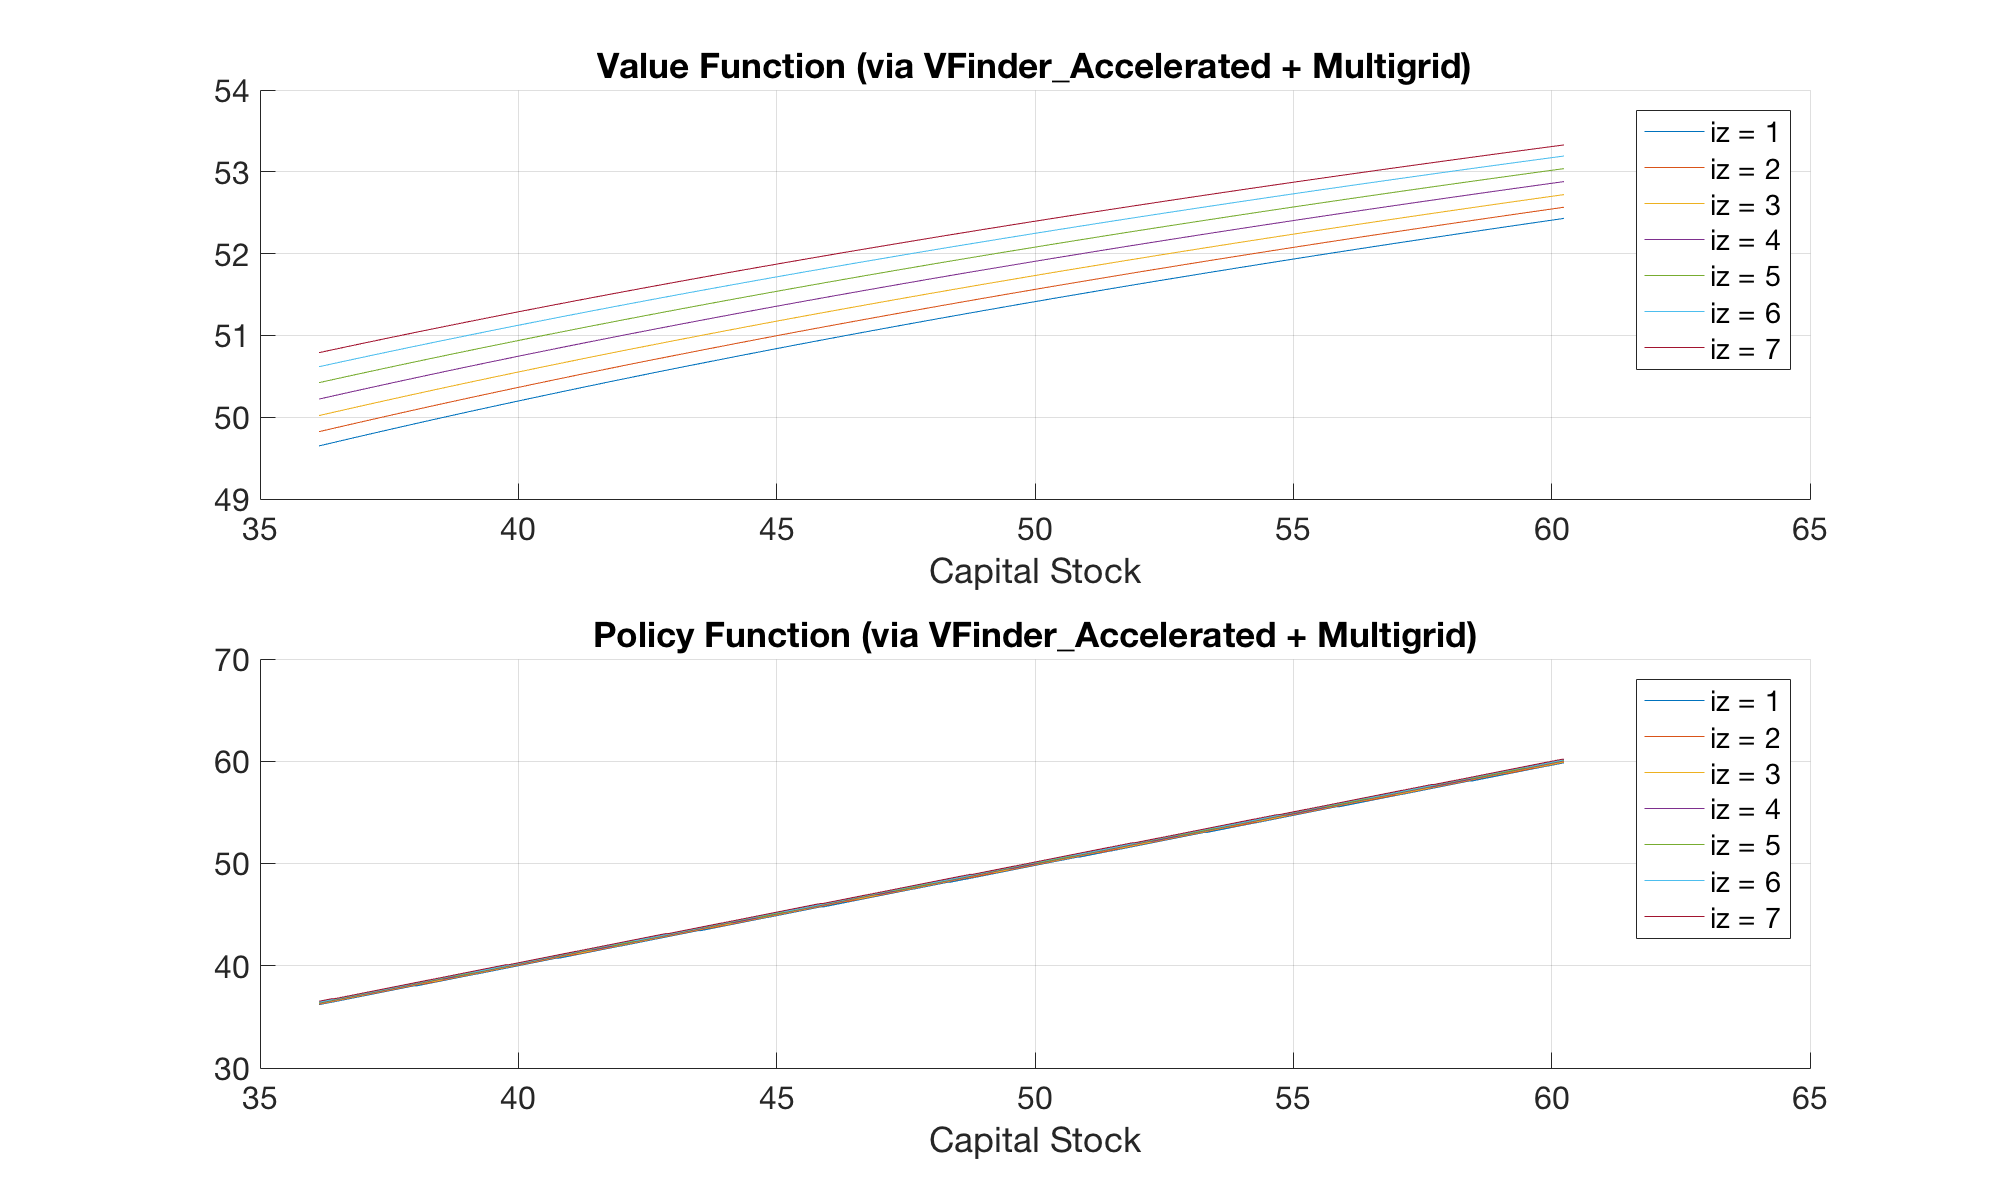
\includegraphics[scale = 0.22]{multigrid}
	\end{figure}
\end{problema}
	
\begin{problema}
	O método do grid endógeno mostrou-se também poderoso, ainda que tenha tido performance um pouco pior do que o multigrid. O algoritmo convergiu em 1.66 segundos, o que representa uma significativa melhora com respeito ao método do acelerador e da força bruta, no entanto.
	
	Como pode ser visto a partir da Equação de Euler derivada no Problema 2, dado o grid exógeno para $k'$ e um chute para a função política do consumo, não podemos inverter o lado esquerdo diretamente e encontrar o valor de $k_{egm}$ do grid endógeno pois a função $zk^{\alpha} + (1-\delta)k$ não admite inversa analítica trivial em $k$, ponto a ponto em $z$. A saída que encontrei foi inverter $m(k) =  zk^{\alpha} + (1-\delta)k$ numericamente, dado um valor de $z$. Fiz isto através da função $\texttt{polyfit}$ do MATLAB, usando um polinômio de grau 4.
	
	Uma vez que não há teoremas gerais com respeito à convergência do método do grid endógeno, computei os Euler Errors para checar a qualidade da aproximação. O erro médio foi de $-3.033$, o que considero satisfatório. A figure a seguir mostra a função política do capital e os Euler Errors encontrados:
	\begin{figure}[h!]
		\centering
		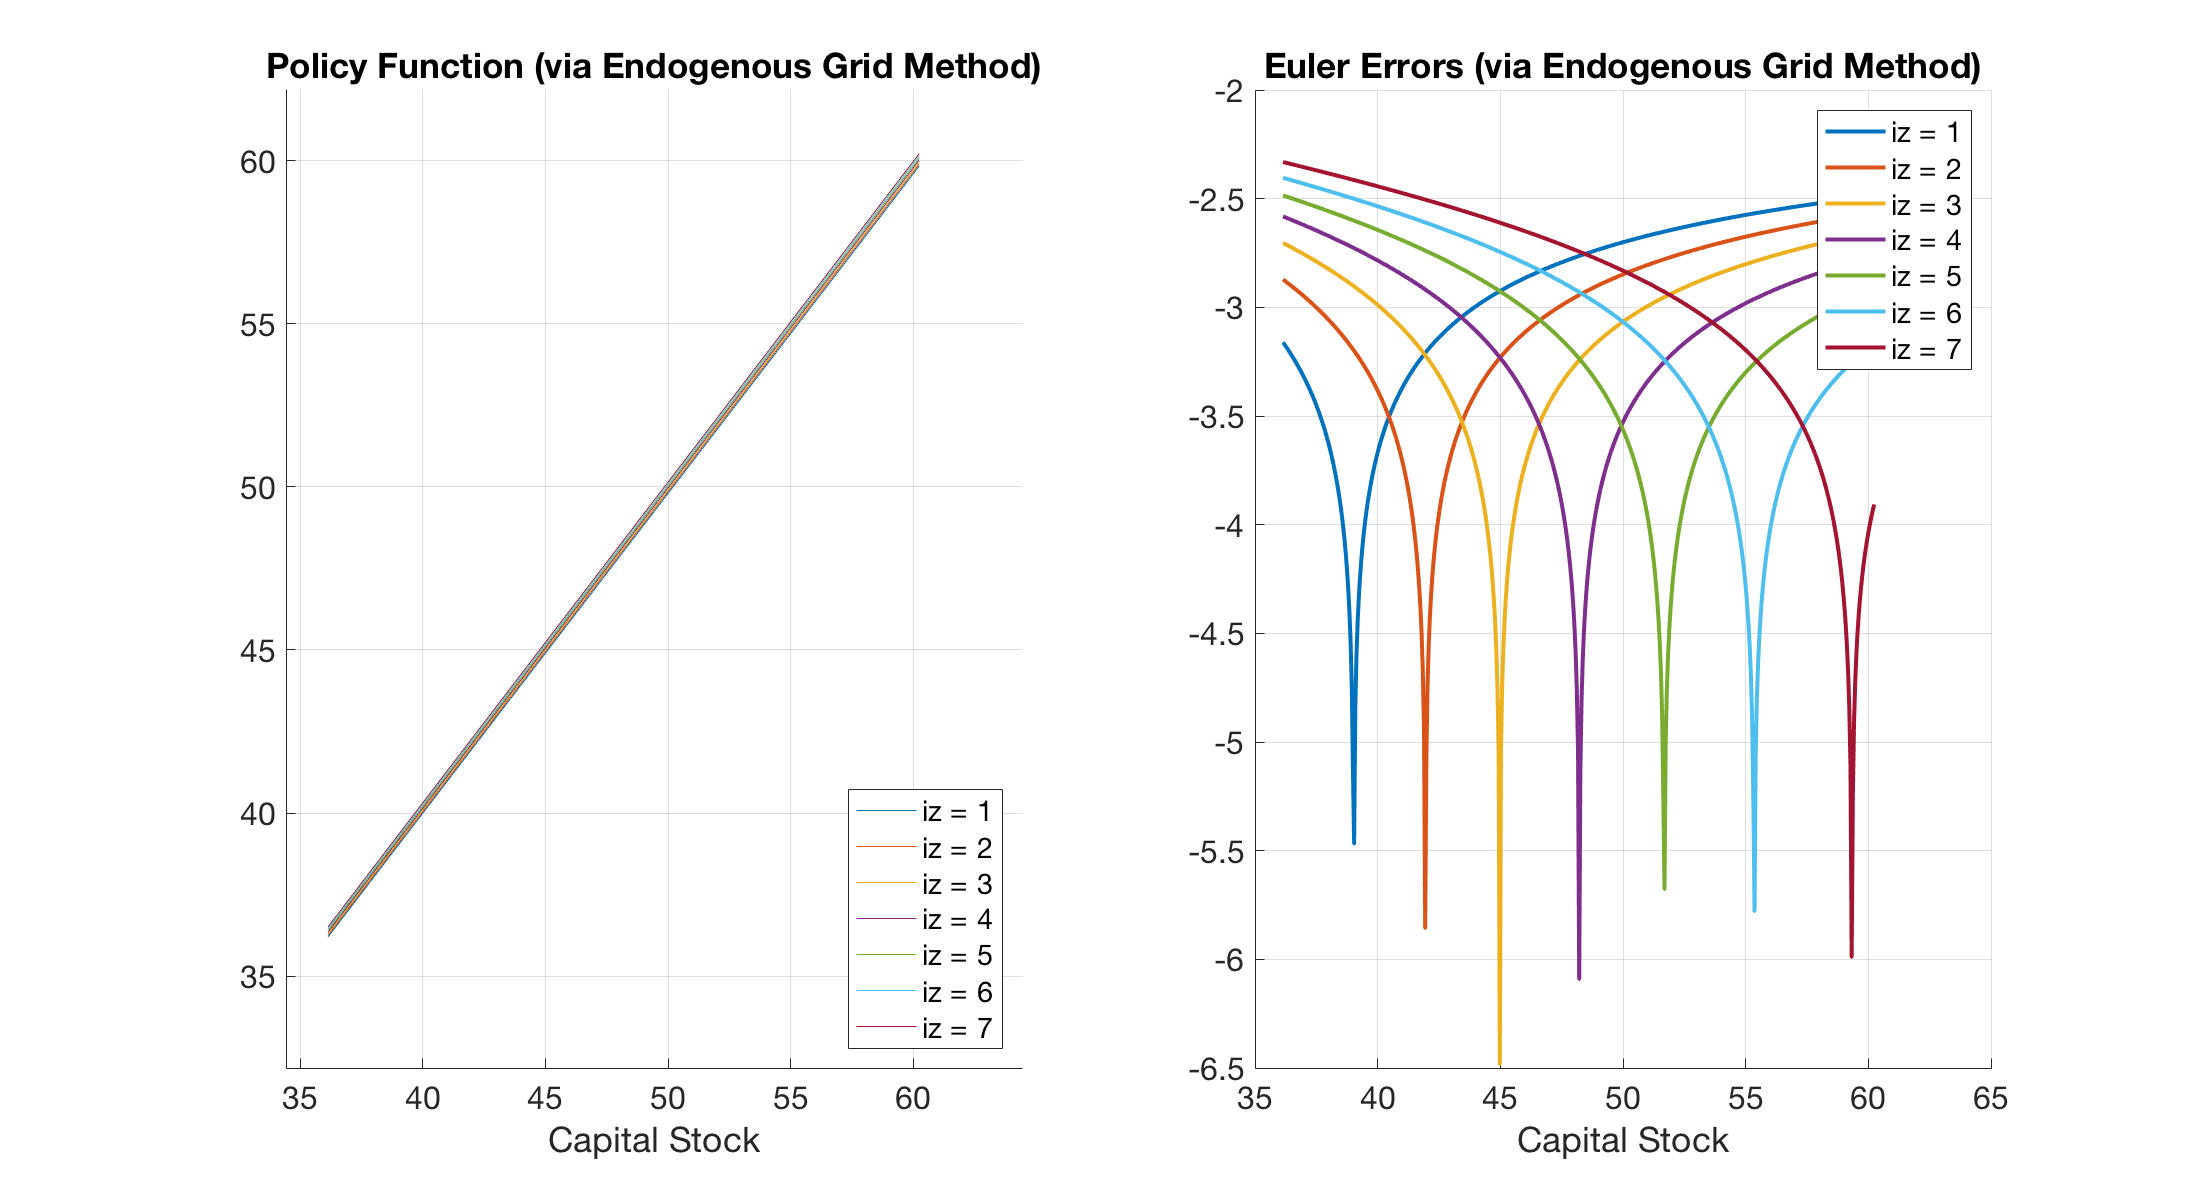
\includegraphics[scale = 0.22]{EE.png}
	\end{figure}
	
	A qualidade da aproximação é tanto melhor quanto mais próximo se estiver do capital de estado estacionário sem incerteza, para cada $z$ fixo. De fato, nos pontos de maior precisão, os Euler Errors ficaram ao redor de -6, valor considerado satisfatório pelos slides. Nos pontos em que a aproximação se mostrou pior, os Euler Errors se mantiveram ao redor de -2.5. Levando em conta a escala logarítmica, a interpretação nestes casos é de que estamos errando o valor do consumo ótimo em \$1 a cada $10^{-2.5} \approx \$ 316$ gastos, um erro de aproximadamente $0.32\%$. 
\end{problema}
\end{document}
